\iffalse
\documentclass[12pt]{article}
\usepackage{graphicx}
\usepackage{commath}
\usepackage{gensymb}
\usepackage{float}

\begin{document}
\begin{center}
\textbf\large{CHAPTER-7 \\ COORDINATE GEOMETRY}
\end{center}

\section{EXERCISE - 7.1}
\fi
\begin{enumerate}[label=\thesection.\arabic*,ref=\thesection.\theenumi]
\numberwithin{equation}{enumi}
\numberwithin{figure}{enumi}
\numberwithin{table}{enumi}
\item Find the distances between the following pairs of points:
\begin{enumerate}
\item $(2,3),(4,1)$
\item $(-5,7),(-1,3)$
\item $(a,b),(-a,-b)$
\end{enumerate}
		\iffalse
\documentclass[12pt]{article}
\usepackage{graphicx}
\usepackage{amsmath}
\usepackage{mathtools}
\usepackage{gensymb}

\newcommand{\mydet}[1]{\ensuremath{\begin{vmatrix}#1\end{vmatrix}}}
\providecommand{\brak}[1]{\ensuremath{\left(#1\right)}}
\providecommand{\norm}[1]{\left\lVert#1\right\rVert}
\newcommand{\solution}{\noindent \textbf{Solution: }}
\newcommand{\myvec}[1]{\ensuremath{\begin{pmatrix}#1\end{pmatrix}}}
\let\vec\mathbf

\begin{document}
\begin{center}
\textbf\large{CHAPTER-7 \\ COORDINATE GEOMETRY}
\end{center}
\section*{Excercise 7.1}

Q1. Find the distance between the following pairs of points :
\begin{enumerate}
	\item $\brak{2,3}, \brak{4,1}$ 
	\item $\brak{-5,7}, \brak{-1,3}$
	\item $\brak{a,b}, \brak{-a,-b}$
\end{enumerate}
\fi
\solution
\begin{enumerate}
\item The coordinates are given as
	\begin{align}
	\vec{A} = \myvec{
		2\\
		3\\
		},
		\vec{B} &= \myvec{
		4\\
		1\\
		}
		\\
\implies		\vec{A} - \vec{B} = \myvec{2\\3} - \myvec{4\\1} &= \myvec{-2\\2}		
\\
		\implies		(\vec{A}-\vec{B})^\top (\vec{A}-\vec{B}) &= 8
	\end{align}
	Thus, the desired distance is 
	\begin{align}
		d=\norm{\vec{A}-\vec{B}} =\sqrt{8}
	\end{align}
	See Fig. \ref{fig:10/7/1/1Fig}.
\item The coordinates are given as
	\begin{align}
	\vec{C} = \myvec{
		-5\\
		7\\
		},
		\vec{D} &= \myvec{
		-1\\
		3\\
		}
\implies		\vec{C} - \vec{D} = \myvec{-5\\7} - \myvec{-1\\3} &= \myvec{-4\\4}		
		\\
		\implies		(\vec{C}-\vec{D})^\top (\vec{C}-\vec{D}) &= 32
	\end{align}
Thus,	
	\begin{align}
		d=\norm{\vec{C}-\vec{D}}
 =4\sqrt{2}
\end{align}	
	See Fig. \ref{fig:10/7/1/1Fig}.
%	
\item The coordinates are given as
	\begin{align}
	\vec{E} = \myvec{
		a\\
		b\\
		},
		\vec{F} &= \myvec{
		-a\\
		-b\\
		}
		\implies		\vec{E} - \vec{F} = \myvec{a\\b} - \myvec{-a\\-b} &= \myvec{2a\\2b}		
		\\
		\implies
		(\vec{E}-\vec{F})^\top (\vec{E}-\vec{F}) = 4a^2+4b^2 
	\end{align}
Thus,	
	\begin{align}
		d=\norm{\vec{E}-\vec{F}} =
2\sqrt{a^2+b^2}
\end{align}	
See  
Fig. \ref{fig:10/7/1/1Fig} for 
$ a=1,b=2$ 
\begin{figure}[!h]
	\begin{center} 
	    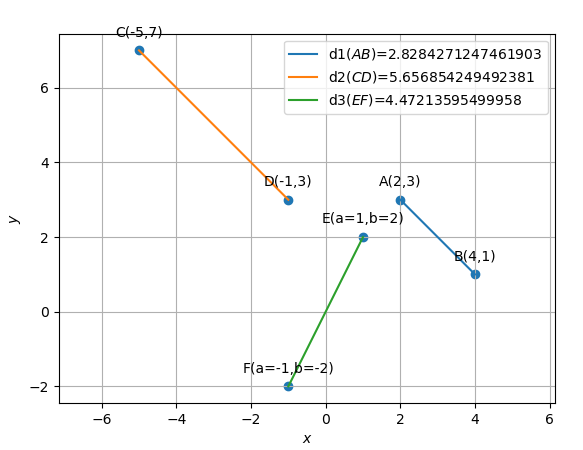
\includegraphics[width=\columnwidth]{chapters/10/7/1/1/figs/graph.png}
	\end{center}
\caption{}
\label{fig:10/7/1/1Fig}
\end{figure}
\end{enumerate}

\item Find the distance between the points $(0,0)$ and $ (36,15)$.
	\\
		\solution
		\iffalse
\documentclass[journal,12pt,twocolumn]{IEEEtran}
\usepackage{graphicx}
\graphicspath{{./chapters/10/7/1/2/figs/}}{}
\usepackage{amsmath,amssymb,amsfonts,amsthm}
\newcommand{\myvec}[1]{\ensuremath{\begin{pmatrix}#1\end{pmatrix}}}
\providecommand{\norm}[1]{\lVert#1\rVert}
\usepackage{listings}
\usepackage{watermark}
\usepackage{titlesec}
\usepackage{caption}
\let\vec\mathbf
\lstset{
frame=single, 
breaklines=true,
columns=fullflexible
}
\thiswatermark{\centering \put(0,-105.0){
\includegraphics[scale=0.15]{/sdcard/IITH/vector/chapters/10/7/1/2/figs/logo2.png}} }
\title{\mytitle}
\title{
Assignment - Vector
}
\author{Surajit Sarkar}
\begin{document}
\maketitle
\tableofcontents
\bigskip
\section{\textbf{Problem}}
Find the distance between the point(0,0) and (36,15).Can you now find the distance between the two towns A and B discussed in Section 7.2
\section{\textbf{Solution}}
\fi
Let
\begin{align}
\vec{A}&=\myvec{0 \\ 0}  
\Vec{B}=\myvec{36 \\ 15} \\ 
\implies 
\vec{d}&=\norm{\vec{A}-\vec{B}}=\sqrt{\myvec{\vec{A}-\vec{B}}^T\myvec{\vec{A}-\vec{B}}} \\
&=39
\end{align}
See Fig. 
\ref{fig:10/7/1/2vec}.
\begin{figure}[!h]
\centering
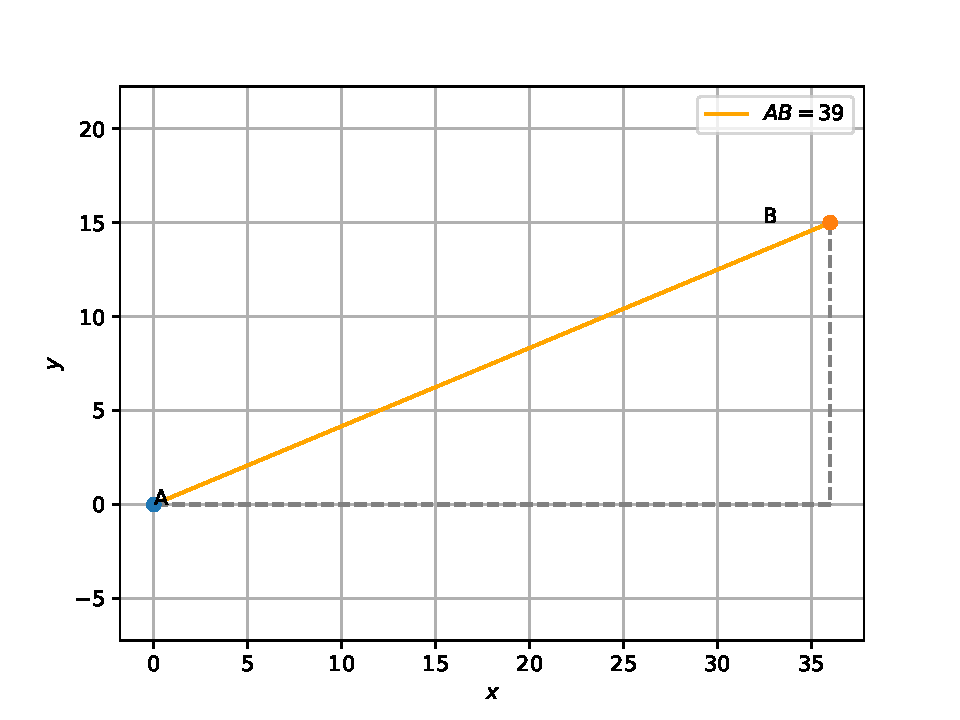
\includegraphics[width=\columnwidth]{chapters/10/7/1/2/figs/vec.pdf}
\caption{}
\label{fig:10/7/1/2vec}
\end{figure}

\item Determine if the points $(1,5),(2,3)$ and $(-2,-11)$ are collinear.
	\\
		\iffalse
\documentclass[12pt]{article}
\usepackage{graphicx}
\usepackage[none]{hyphenat}
\usepackage{graphicx}
\usepackage{listings}
\usepackage[english]{babel}
\usepackage{graphicx}
\usepackage{caption} 
\usepackage{hyperref}
\usepackage{booktabs}
\usepackage{array}
\usepackage{amsmath}   % for having text in math mode
\usepackage{extarrows} % for Row operations arrows
\usepackage{listings}
\lstset{
  frame=single,
  breaklines=true
}
  
%Following 2 lines were added to remove the blank page at the beginning
\usepackage{atbegshi}% http://ctan.org/pkg/atbegshi
\AtBeginDocument{\AtBeginShipoutNext{\AtBeginShipoutDiscard}}


%New macro definitions
\newcommand{\mydet}[1]{\ensuremath{\begin{vmatrix}#1\end{vmatrix}}}
\providecommand{\brak}[1]{\ensuremath{\left(#1\right)}}
\providecommand{\norm}[1]{\left\lVert#1\right\rVert}
\newcommand{\solution}{\noindent \textbf{Solution: }}
\newcommand{\myvec}[1]{\ensuremath{\begin{pmatrix}#1\end{pmatrix}}}
\let\vec\mathbf

\begin{document}

\begin{center}
\title{\textbf{Properties of Triangles}}
\date{\vspace{-5ex}} %Not to print date automatically
\maketitle
\end{center}
\setcounter{page}{1}

\section{10$^{th}$ Maths - Chapter 7}
This is Problem-3 from Exercise 7.1
\begin{enumerate}
\item Determine if the points $(1,5), (2,3), \text{ and } (-2,-11)$ are collinear.  \\
	\fi
\solution 
 We know that points $\vec{A}, \vec{B} \text{ and } \vec{C}$ are collinear, if
\begin{align}
  \label{eq:10/7/1/31}
\text{rank}\myvec{ 
	\vec{A}^\top \\ 
	\vec{B}^\top \\ 
	\vec{C}^\top 
}    &=  1 
\end{align}
Since
\begin{align}
	\myvec{ \vec{A}^\top \\ 
			\vec{B}^\top \\ 
			\vec{C}^\top 
} =   		\myvec{
        		1 & 5 \\
        		2 & 3 \\
        		-2 & -11 
}
\\
\xleftrightarrow[{R_3\rightarrow R_3+2R_1}]{{R_2\rightarrow R_2-2R_1}}  \myvec{
  1 & 5 \\
  0 & -7 \\
  0 & -1 
}    
\xleftrightarrow[]{{R_3\rightarrow R_3-\frac{1}{7}R_2}}  \myvec{
  1 & 5 \\
  0 & -7 \\
  0 & 0 
},
\end{align}
 the rank of the matrix is 2. From \eqref{eq:10/7/1/31}, the points are not collinear.  This is verified by Fig.  
 \ref{fig:10/7/1/3Fig1}, where the given points constitute a triangle and not a line.
\begin{figure}[!h]
	\begin{center}
		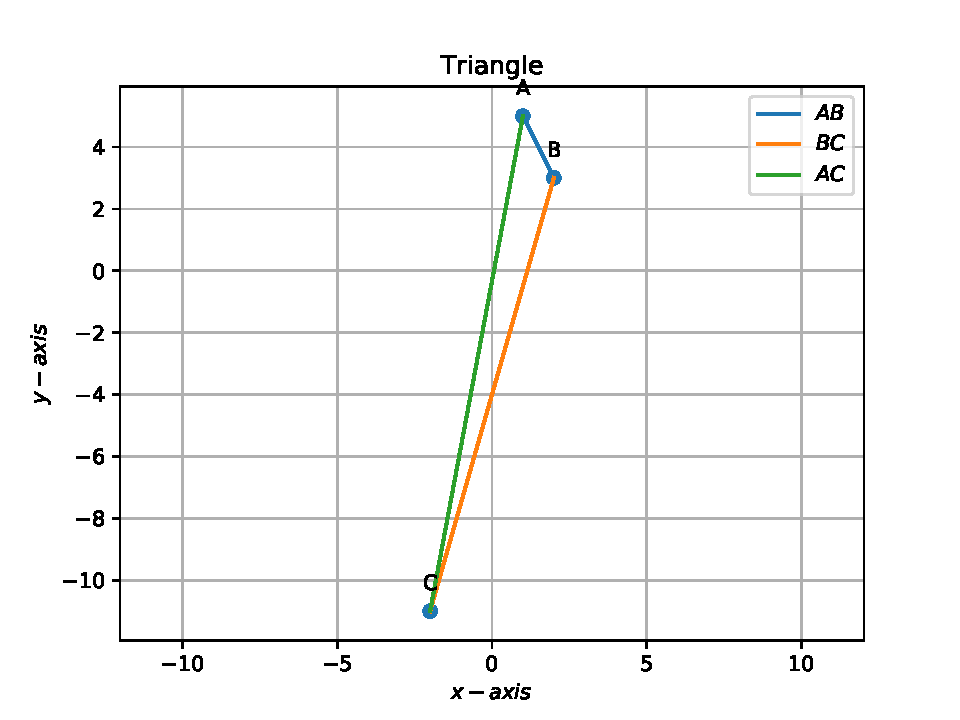
\includegraphics[width=\columnwidth]{chapters/10/7/1/3/figs/problem3.pdf}
	\end{center}
\caption{}
\label{fig:10/7/1/3Fig1}
\end{figure}


\item Check whether$(5,-2),(6,4)$ and $(7,-2)$ are the vertices of an isosceles triangle.
	\iffalse
\item  In a classroom, 4 friends are seated at the points A,B,C and D as shown in Fig. 7.8, Champa and Chameli walk in to the class and after observing for a few minutes Champa asks Chameli,"Dont't you think ABCD is a square?" Chameli disagrees,Using distance formula, find which of them is correct.

\begin{figure}[!h]
\centering
  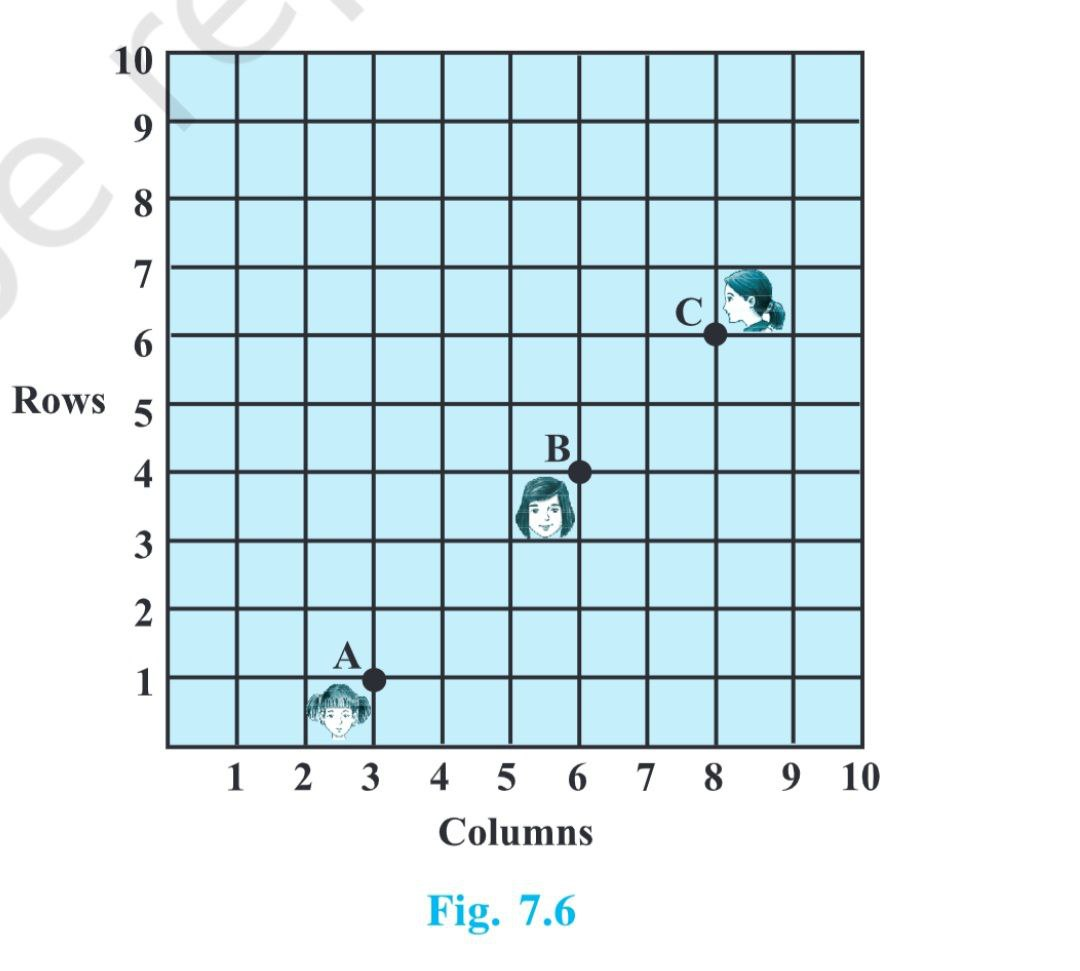
\includegraphics[width=\columnwidth]{canvas.jpg}
 \caption{}
\label{fig:10/7/4/8Fig3}
\end{figure}
\fi
\item Name the type of quadrilateral formed,if any,by the following points,and give reasons for your answer
\begin{enumerate}
\item $(-1,-2),(1,0),(-1,2),(-3,0)$
\item $(-3,5),(-3,1),(0,3),(-1,-4)$
\item $(4,5),(7,6),(4,3),(1,2)$
\end{enumerate}
\solution
		\iffalse
\documentclass[12pt]{article}
\usepackage{graphicx}
\usepackage{amsmath}
\usepackage{mathtools}
\usepackage{gensymb}

\newcommand{\mydet}[1]{\ensuremath{\begin{vmatrix}#1\end{vmatrix}}}
\providecommand{\brak}[1]{\ensuremath{\left(#1\right)}}
\providecommand{\norm}[1]{\left\lVert#1\right\rVert}
\newcommand{\solution}{\noindent \textbf{Solution: }}
\newcommand{\myvec}[1]{\ensuremath{\begin{pmatrix}#1\end{pmatrix}}}
\let\vec\mathbf

\begin{document}
\begin{center}
\textbf\large{CHAPTER-7 \\ COORDINATE GEOMETRY}

\end{center}
\section*{Excercise 7.1}

Q6.Name the type of quadilateral formed,if any, by the following points, and give reasons for your answer:
\begin{enumerate}
	\item $\brak{-1,-2}, \brak{1,0}, \brak{-1,2}, \brak{-3,0}$ 
	\item $\brak{-3,5}, \brak{3,1}, \brak{0,3}, \brak{-1,-4}$
	\item $\brak{4,5}, \brak{7,6}, \brak{4,3}, \brak{1,2}$
\end{enumerate}
\solution
\fi
\begin{enumerate}
\item The coordinates are given as
	\begin{align}
	\vec{A} = \myvec{
		-1\\
		-2\\
		},
	\vec{B} = \myvec{
		1\\
		0\\
		},
	\vec{C} = \myvec{
		-1\\
		2\\
		} \text{ and }
	\vec{D} = \myvec{
		-3\\
		0\\
		}
	\end{align}
	\begin{align}
		\vec{B} - \vec{A} &= \myvec{1\\0} - \myvec{-1\\-2} = \myvec{2\\2}\\
		\vec{C} - \vec{B} &= \myvec{-1\\2} - \myvec{1\\0} = \myvec{-2\\2}\\
		\vec{C} - \vec{D} &= \myvec{-1\\2} - \myvec{-3\\0} = \myvec{2\\2}\\
		\vec{D} - \vec{A} &= \myvec{-3\\0} - \myvec{-1\\-2} = \myvec{-2\\2}
	\end{align}
	\begin{align}	
		\vec{C} - \vec{A} &= \myvec{-1\\2} - \myvec{-1\\-2} = \myvec{0\\4}\\
		\vec{D} - \vec{B} &= \myvec{-3\\0} - \myvec{1\\0} = \myvec{-4\\0}
	\end{align}
	\begin{align}	
		\vec{B}-\vec{A} = \vec{C}-\vec{D} \text{ and } \vec{C}-\vec{B} = \vec{D}-\vec{A}.
	\end{align}
	Hence, $ABCD$ is a parallelogram.
	\begin{enumerate}
		\item Now checking if the adjacent sides are orthogonal to each other
	\begin{align}
		(\vec{B}-\vec{A})^\top (\vec{C}-\vec{B}) = \myvec{2&2} \myvec{-2\\2} = -4+4 = 0
	\end{align}
		\item Now checking if the diagonals are also orthogonal then it is a square else a rectangle.
	\end{enumerate}	
	\begin{align}
		(\vec{C}-\vec{A})^\top (\vec{D}-\vec{B}) = \myvec{0&4} \myvec{-4\\0} = 0
	\end{align}
	Hence the diagonals are orthogonal to each other.

	So, we can conclude that $ABCD$ is a square.

	As shown in Figure \ref{fig:10/7/1/6/Fig1} we can see that $ABCD$ is a square hence we can conclude that our theoritical result is verified.
 
\begin{figure}[!h]
	\begin{center} 
	    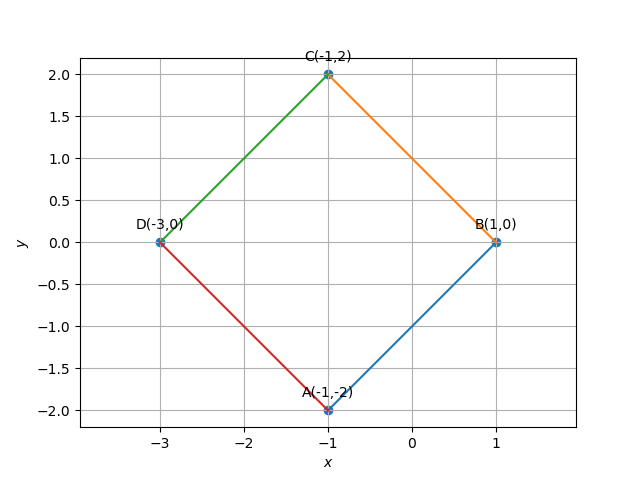
\includegraphics[width=\columnwidth]{chapters/10/7/1/6/figs/quad1}
	\end{center}
\caption{}
\label{fig:10/7/1/6/Fig1}
\end{figure}

\item The coordinates are given as
	\begin{align}
	\vec{A} = \myvec{
		-3\\
		5\\
		},
	\vec{B} = \myvec{
		3\\
		1\\
		},
	\vec{C} = \myvec{
		0\\
		3\\
		} \text{ and }
	\vec{D} = \myvec{
		-1\\
		-4\\
		}
	\end{align}
	\begin{align}
		\vec{B} - \vec{A} &= \myvec{3\\1} - \myvec{-3\\5} = \myvec{6\\-4}\\
		\vec{C} - \vec{B} &= \myvec{0\\3} - \myvec{3\\1} = \myvec{-3\\2}\\
		\vec{C} - \vec{D} &= \myvec{0\\3} - \myvec{-1\\-4} = \myvec{1\\7}\\
		\vec{D} - \vec{A} &= \myvec{-1\\-4} - \myvec{-3\\5} = \myvec{2\\-9}
	\end{align}
	\begin{align}
		\vec{C} - \vec{A} &= \myvec{0\\3} - \myvec{-3\\5} = \myvec{3\\-2}\\
		\vec{D} - \vec{B} &= \myvec{-1\\-4} - \myvec{3\\1} = \myvec{-4\\-5}
	\end{align}
	\begin{align}
	\vec{B}-\vec{A} \neq \vec{C}-\vec{D} \text{ and } \vec{C}-\vec{B} \neq \vec{D}-\vec{A},
	\end{align}
	Hence, $ABCD$ is not a parallelogram, it can be a irregular quadilateral.
	\begin{enumerate}
		\item Now to check if any three points are collinear,

	if rank of $\myvec{\vec{B}-\vec{A} & \vec{C}-\vec{B}} = 1$ then points are collinear

	Forming the collinearity matrix
	\begin{align}
		\myvec{6&-3\\-4&2} \xleftrightarrow{R_{2}\rightarrow R_{2}+\frac{2}{3}R_{1}}= \myvec{6&-3\\0&0}
	\end{align}
	\end{enumerate}
	Hence, rank = 1

	Since none of the opposite sides are parallel to each other and three points are collinear so these does not form a quadilateral.

	As shown in Figure \ref{fig:10/7/1/6/Fig2} we can see that $ABCD$ does not form a quadilateral and three points are collinear hence, our theoritical result is verified.
	
\begin{figure}[!h]
	\begin{center} 
	    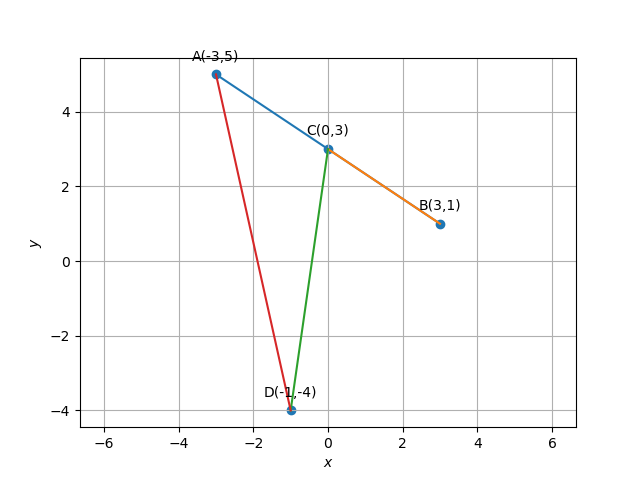
\includegraphics[width=\columnwidth]{chapters/10/7/1/6/figs/quad2}
	\end{center}
\caption{}
\label{fig:10/7/1/6/Fig2}
\end{figure}
	
\item The coordinates are given as
	\begin{align}
	\vec{A} = \myvec{
		4\\
		5\\
		},
	\vec{B} = \myvec{
		7\\
		6\\
		},
	\vec{C} = \myvec{
		4\\
		3\\
		} \text{ and }
	\vec{D} = \myvec{
		1\\
		2\\
		}
	\end{align}
	\begin{align}
		\vec{B} - \vec{A} &= \myvec{7\\6} - \myvec{4\\5} = \myvec{3\\1}\\
		\vec{C} - \vec{B} &= \myvec{4\\3} - \myvec{7\\6} = \myvec{-3\\-3}\\
		\vec{C} - \vec{D} &= \myvec{4\\3} - \myvec{1\\2} = \myvec{3\\1}\\
		\vec{D} - \vec{A} &= \myvec{1\\2} - \myvec{4\\5} = \myvec{-3\\-3}
	\end{align}
	\begin{align}
		\vec{C} - \vec{A} &= \myvec{4\\3} - \myvec{4\\5} = \myvec{0\\-2}\\
		\vec{D} - \vec{B} &= \myvec{1\\2} - \myvec{7\\6} = \myvec{-6\\-4}
	\end{align}
	\begin{align}
		\vec{B}-\vec{A} = \vec{C}-\vec{D} \text{ and } \vec{C}-\vec{B} = \vec{D}-\vec{A},
	\end{align}
	Hence, $ABCD$ is a parallelogram.
	\begin{enumerate}
		\item Now checking if the adjacent sides are orthogonal to each other
	\begin{align}
		(\vec{B}-\vec{A})^\top (\vec{C}-\vec{B}) = \myvec{3&1} \myvec{-3\\-3} = -9-3 = -12
	\end{align}
	Since inner product is not zero so adjacent sides are not orthogonal.

	Hence, we can say that $ABCD$ is neither a rectangle nor a square.

		\item Now checking if the diagonals are orthogonal then it is a Rhombus.
	\begin{align}
		(\vec{C}- \vec{A})^\top (\vec{D}-\vec{B}) = \myvec{0&-2} \myvec{-6\\-4} = 0+8 = 8
	\end{align}
	\end{enumerate}		
	Hence the diagonals are also not orthogonal so we conclude that $ABCD$ is a parallelogram.

	As shown in Figure \ref{fig:10/7/1/6/Fig3} we can see that $ABCD$ forms a parallelogram hence, our theoritical result is verified.

\begin{figure}[!h]
	\begin{center} 
	    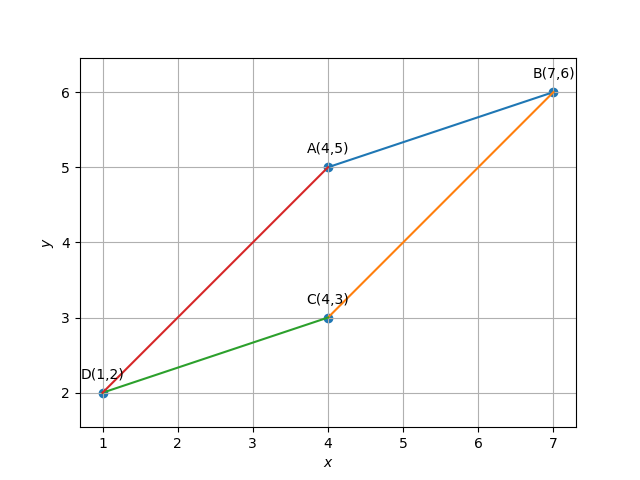
\includegraphics[width=\columnwidth]{chapters/10/7/1/6/figs/quad3}
	\end{center}
\caption{}
\label{fig:10/7/1/6/Fig3}
\end{figure}
\end{enumerate}



\item Find the point on the x-axis which is equidistant from $(2,-5)$ and $(-2,9)$.
	\\
\solution
		\iffalse
\documentclass[12pt]{article}
\usepackage{graphicx}
%\documentclass[journal,12pt,twocolumn]{IEEEtran}
\usepackage[none]{hyphenat}
\usepackage{graphicx}
\usepackage{listings}
\usepackage[english]{babel}
\usepackage{graphicx}
\usepackage{caption} 
\usepackage{hyperref}
\usepackage{booktabs}
\def\inputGnumericTable{}
\usepackage{color}                                            %%
    \usepackage{array}                                            %%
    \usepackage{longtable}                                        %%
    \usepackage{calc}                                             %%
    \usepackage{multirow}                                         %%
    \usepackage{hhline}                                           %%
    \usepackage{ifthen}
\usepackage{array}
\usepackage{amsmath}   % for having text in math mode
\usepackage{listings}
\lstset{
language=tex,
frame=single, 
breaklines=true
}
  
%Following 2 lines were added to remove the blank page at the beginning
\usepackage{atbegshi}% http://ctan.org/pkg/atbegshi
\AtBeginDocument{\AtBeginShipoutNext{\AtBeginShipoutDiscard}}
%


%New macro definitions
\newcommand{\mydet}[1]{\ensuremath{\begin{vmatrix}#1\end{vmatrix}}}
\providecommand{\brak}[1]{\ensuremath{\left(#1\right)}}
\providecommand{\norm}[1]{\left\lVert#1\right\rVert}
\newcommand{\solution}{\noindent \textbf{Solution: }}
\newcommand{\myvec}[1]{\ensuremath{\begin{pmatrix}#1\end{pmatrix}}}
\let\vec\mathbf

\begin{document}

\begin{center}
\title{\textbf{Coordinate Geometry}}
\date{\vspace{-5ex}} %Not to print date automatically
\maketitle
\end{center}

\setcounter{page}{1}



\section*{10$^{th}$ Maths - Chapter 7}

This is Problem-7 from Exercise 7.1

\begin{enumerate}

\item The point on the $x$-axis which is equidistant from $\myvec{2 \\ -5}$ and $\myvec{-2\\9}$\\
\solution \\
\fi
		The input parameters for this problem are available in Table \ref{tab:10/7/1/7Table-1}
\begin{table}[ht!]
%%%%%%%%%%%%%%%%%%%%%%%%%%%%%%%%%%%%%%%%%%%%%%%%%%%%%%%%%%%%%%%%%%%%%%
%%                                                                  %%
%%  This is the header of a LaTeX2e file exported from Gnumeric.    %%
%%                                                                  %%
%%  This file can be compiled as it stands or included in another   %%
%%  LaTeX document. The table is based on the longtable package so  %%
%%  the longtable options (headers, footers...) can be set in the   %%
%%  preamble section below (see PRAMBLE).                           %%
%%                                                                  %%
%%  To include the file in another, the following two lines must be %%
%%  in the including file:                                          %%
%%        \def\inputGnumericTable{}                                 %%
%%  at the beginning of the file and:                               %%
%%        \input{name-of-this-file.tex}                             %%
%%  where the table is to be placed. Note also that the including   %%
%%  file must use the following packages for the table to be        %%
%%  rendered correctly:                                             %%
%%    \usepackage[latin1]{inputenc}                                 %%
%%    \usepackage{color}                                            %%
%%    \usepackage{array}                                            %%
%%    \usepackage{longtable}                                        %%
%%    \usepackage{calc}                                             %%
%%    \usepackage{multirow}                                         %%
%%    \usepackage{hhline}                                           %%
%%    \usepackage{ifthen}                                           %%
%%  optionally (for landscape tables embedded in another document): %%
%%    \usepackage{lscape}                                           %%
%%                                                                  %%
%%%%%%%%%%%%%%%%%%%%%%%%%%%%%%%%%%%%%%%%%%%%%%%%%%%%%%%%%%%%%%%%%%%%%%



%%  This section checks if we are begin input into another file or  %%
%%  the file will be compiled alone. First use a macro taken from   %%
%%  the TeXbook ex 7.7 (suggestion of Han-Wen Nienhuys).            %%
\def\ifundefined#1{\expandafter\ifx\csname#1\endcsname\relax}


%%  Check for the \def token for inputed files. If it is not        %%
%%  defined, the file will be processed as a standalone and the     %%
%%  preamble will be used.                                          %%
\ifundefined{inputGnumericTable}

%%  We must be able to close or not the document at the end.        %%
	\def\gnumericTableEnd{\end{document}}


%%%%%%%%%%%%%%%%%%%%%%%%%%%%%%%%%%%%%%%%%%%%%%%%%%%%%%%%%%%%%%%%%%%%%%
%%                                                                  %%
%%  This is the PREAMBLE. Change these values to get the right      %%
%%  paper size and other niceties.                                  %%
%%                                                                  %%
%%%%%%%%%%%%%%%%%%%%%%%%%%%%%%%%%%%%%%%%%%%%%%%%%%%%%%%%%%%%%%%%%%%%%%

	\documentclass[12pt%
			  %,landscape%
                    ]{report}
       \usepackage[latin1]{inputenc}
       \usepackage{fullpage}
       \usepackage{color}
       \usepackage{array}
       \usepackage{longtable}
       \usepackage{calc}
       \usepackage{multirow}
       \usepackage{hhline}
       \usepackage{ifthen}

	\begin{document}


%%  End of the preamble for the standalone. The next section is for %%
%%  documents which are included into other LaTeX2e files.          %%
\else

%%  We are not a stand alone document. For a regular table, we will %%
%%  have no preamble and only define the closing to mean nothing.   %%
    \def\gnumericTableEnd{}

%%  If we want landscape mode in an embedded document, comment out  %%
%%  the line above and uncomment the two below. The table will      %%
%%  begin on a new page and run in landscape mode.                  %%
%       \def\gnumericTableEnd{\end{landscape}}
%       \begin{landscape}


%%  End of the else clause for this file being \input.              %%
\fi

%%%%%%%%%%%%%%%%%%%%%%%%%%%%%%%%%%%%%%%%%%%%%%%%%%%%%%%%%%%%%%%%%%%%%%
%%                                                                  %%
%%  The rest is the gnumeric table, except for the closing          %%
%%  statement. Changes below will alter the table's appearance.     %%
%%                                                                  %%
%%%%%%%%%%%%%%%%%%%%%%%%%%%%%%%%%%%%%%%%%%%%%%%%%%%%%%%%%%%%%%%%%%%%%%

\providecommand{\gnumericmathit}[1]{#1} 
%%  Uncomment the next line if you would like your numbers to be in %%
%%  italics if they are italizised in the gnumeric table.           %%
%\renewcommand{\gnumericmathit}[1]{\mathit{#1}}
\providecommand{\gnumericPB}[1]%
{\let\gnumericTemp=\\#1\let\\=\gnumericTemp\hspace{0pt}}
 \ifundefined{gnumericTableWidthDefined}
        \newlength{\gnumericTableWidth}
        \newlength{\gnumericTableWidthComplete}
        \newlength{\gnumericMultiRowLength}
        \global\def\gnumericTableWidthDefined{}
 \fi
%% The following setting protects this code from babel shorthands.  %%
 \ifthenelse{\isundefined{\languageshorthands}}{}{\languageshorthands{english}}
%%  The default table format retains the relative column widths of  %%
%%  gnumeric. They can easily be changed to c, r or l. In that case %%
%%  you may want to comment out the next line and uncomment the one %%
%%  thereafter                                                      %%
\providecommand\gnumbox{\makebox[0pt]}
%%\providecommand\gnumbox[1][]{\makebox}

%% to adjust positions in multirow situations                       %%
\setlength{\bigstrutjot}{\jot}
\setlength{\extrarowheight}{\doublerulesep}

%%  The \setlongtables command keeps column widths the same across  %%
%%  pages. Simply comment out next line for varying column widths.  %%
\setlongtables

\setlength\gnumericTableWidth{%
	53pt+%
	53pt+%
	82pt+%
	53pt+%
0pt}
\def\gumericNumCols{4}
\setlength\gnumericTableWidthComplete{\gnumericTableWidth+%
         \tabcolsep*\gumericNumCols*2+\arrayrulewidth*\gumericNumCols}
\ifthenelse{\lengthtest{\gnumericTableWidthComplete > \linewidth}}%
         {\def\gnumericScale{1*\ratio{\linewidth-%
                        \tabcolsep*\gumericNumCols*2-%
                        \arrayrulewidth*\gumericNumCols}%
{\gnumericTableWidth}}}%
{\def\gnumericScale{1}}

%%%%%%%%%%%%%%%%%%%%%%%%%%%%%%%%%%%%%%%%%%%%%%%%%%%%%%%%%%%%%%%%%%%%%%
%%                                                                  %%
%% The following are the widths of the various columns. We are      %%
%% defining them here because then they are easier to change.       %%
%% Depending on the cell formats we may use them more than once.    %%
%%                                                                  %%
%%%%%%%%%%%%%%%%%%%%%%%%%%%%%%%%%%%%%%%%%%%%%%%%%%%%%%%%%%%%%%%%%%%%%%

\ifthenelse{\isundefined{\gnumericColA}}{\newlength{\gnumericColA}}{}\settowidth{\gnumericColA}{\begin{tabular}{@{}p{53pt*\gnumericScale}@{}}x\end{tabular}}
\ifthenelse{\isundefined{\gnumericColB}}{\newlength{\gnumericColB}}{}\settowidth{\gnumericColB}{\begin{tabular}{@{}p{53pt*\gnumericScale}@{}}x\end{tabular}}
\ifthenelse{\isundefined{\gnumericColC}}{\newlength{\gnumericColC}}{}\settowidth{\gnumericColC}{\begin{tabular}{@{}p{82pt*\gnumericScale}@{}}x\end{tabular}}
\ifthenelse{\isundefined{\gnumericColD}}{\newlength{\gnumericColD}}{}\settowidth{\gnumericColD}{\begin{tabular}{@{}p{53pt*\gnumericScale}@{}}x\end{tabular}}

	\begin{center}
\begin{tabular}[c]{%
	b{\gnumericColA}%
	b{\gnumericColB}%
	b{\gnumericColC}%
	b{\gnumericColD}%
	}

%%%%%%%%%%%%%%%%%%%%%%%%%%%%%%%%%%%%%%%%%%%%%%%%%%%%%%%%%%%%%%%%%%%%%%
%%  The longtable options. (Caption, headers... see Goosens, p.124) %%
%	\caption{The Table Caption.}             \\	%
% \hline	% Across the top of the table.
%%  The rest of these options are table rows which are placed on    %%
%%  the first, last or every page. Use \multicolumn if you want.    %%

%%  Header for the first page.                                      %%
%	\multicolumn{4}{c}{The First Header} \\ \hline 
%	\multicolumn{1}{c}{colTag}	%Column 1
%	&\multicolumn{1}{c}{colTag}	%Column 2
%	&\multicolumn{1}{c}{colTag}	%Column 3
%	&\multicolumn{1}{c}{colTag}	\\ \hline %Last column
%	\endfirsthead

%%  The running header definition.                                  %%
%	\hline
%	\multicolumn{4}{l}{\ldots\small\slshape continued} \\ \hline
%	\multicolumn{1}{c}{colTag}	%Column 1
%	&\multicolumn{1}{c}{colTag}	%Column 2
%	&\multicolumn{1}{c}{colTag}	%Column 3
%	&\multicolumn{1}{c}{colTag}	\\ \hline %Last column
%	\endhead

%%  The running footer definition.                                  %%
%	\hline
%	\multicolumn{4}{r}{\small\slshape continued\ldots} \\
%	\endfoot

%%  The ending footer definition.                                   %%
%	\multicolumn{4}{c}{That's all folks} \\ \hline 
%	\endlastfoot
%%%%%%%%%%%%%%%%%%%%%%%%%%%%%%%%%%%%%%%%%%%%%%%%%%%%%%%%%%%%%%%%%%%%%%

\hhline{|-|-|-~}
	 \multicolumn{1}{|p{\gnumericColA}|}%
	{\gnumericPB{\centering}\gnumbox{\textbf{Symbol}}}
	&\multicolumn{1}{p{\gnumericColB}|}%
	{\gnumericPB{\centering}\gnumbox{\textbf{Value}}}
	&\multicolumn{1}{p{\gnumericColC}|}%
	{\gnumericPB{\centering}\gnumbox{\textbf{Description}}}
	&
\\
\hhline{|---|~}
	 \multicolumn{1}{|p{\gnumericColA}|}%
	{\gnumericPB{\centering}\gnumbox{$\vec{A}$}}
	&\multicolumn{1}{p{\gnumericColB}|}%
	{\gnumericPB{\centering}\gnumbox{$\myvec{2\\-5}$}}
	&\multicolumn{1}{p{\gnumericColC}|}%
	{\gnumericPB{\centering}\gnumbox{First point}}
	&
\\
\hhline{|---|~}
	 \multicolumn{1}{|p{\gnumericColA}|}%
	{\gnumericPB{\centering}\gnumbox{$\vec{B}$}}
	&\multicolumn{1}{p{\gnumericColB}|}%
	{\gnumericPB{\centering}\gnumbox{$\myvec{-2\\9}$}}
	&\multicolumn{1}{p{\gnumericColC}|}%
	{\gnumericPB{\centering}\gnumbox{Second point}}
	&
\\
\hhline{|---|~}
	 \multicolumn{1}{|p{\gnumericColA}|}%
	{\gnumericPB{\centering}\gnumbox{$\vec{O}$}}
	&\multicolumn{1}{p{\gnumericColB}|}%
	{\gnumericPB{\centering}\gnumbox{$?$}}
	&\multicolumn{1}{p{\gnumericColC}|}%
	{\gnumericPB{\centering}\gnumbox{Desired point}}
	&
\\
\hhline{|-|-|-|~}
\end{tabular}
	\end{center}

\ifthenelse{\isundefined{\languageshorthands}}{}{\languageshorthands{\languagename}}
\gnumericTableEnd

\caption{}
\label{tab:10/7/1/7Table-1}	
\end{table}
%
  If $\vec{O}$ lies on the  $x$-axis and is  equidistant from the points $\vec{A}$ and $\vec{B}$, 
\begin{align}
 \norm{\vec{O}-\vec{A}} &=
\norm{\vec{A}-\vec{B}} 
\\
 \implies \norm{\vec{O}-\vec{A}}^2 &=
\norm{\vec{O}-\vec{B}}^2 
\end{align}
which can be expressed as 
\begin{multline}
%  \label{eq:10/7/1/7norm2d_dist}
 \brak{\vec{O}-\vec{A}}^{\top} \brak{\vec{O}-\vec{A}}=
 \brak{\vec{O}-\vec{B}}^{\top} 
\brak{\vec{O}-\vec{B}}
\\
 \implies \norm{\vec{O}}^2-2{\vec{O}}^{\top}\vec{A} + \norm{\vec{A}}^2
 \\= \norm{\vec{O}}^2-2{\vec{O}}^{\top}\vec{B} + \norm{\vec{B}}^2
\end{multline}
which can be simplified to obtain
%  \eqref{eq:10/7/1/7norm2d_equidist}.
  \begin{align}
   \vec{O} &=
    x\vec{e}_1
  \end{align}
  where 
  \begin{align}
   x &=\frac{\norm{\vec{A}}^2 -\norm{\vec{B}}^2 }{2\brak{\vec{A}-\vec{B}}^{\top }\vec{e}_1
}\label{eq:10/7/1/75}  
  \end{align}
  Substituting from Table \eqref{tab:10/7/1/7Table-1} in \eqref{eq:10/7/1/75},
\begin{align}
 \brak{\vec{A}-\vec{B}}^{\top}=
 \brak{\myvec{2 \\ -5}-\myvec{-2\\9}}^{\top}
	&=\myvec{4 & -14}
	\\
	\norm{\vec{A}}^2 = 21,
	\norm{\vec{B}}^2 &= 85
    \end{align}
yielding $x$ = $ -7$.  Thus, 
		\begin{align}
\vec{O} = \myvec{ -7 \\ 0}.
		\end{align}
		See Fig. 
\ref{fig:10/7/1/7Fig1}.

\begin{figure}[!h]
 \begin{center}
  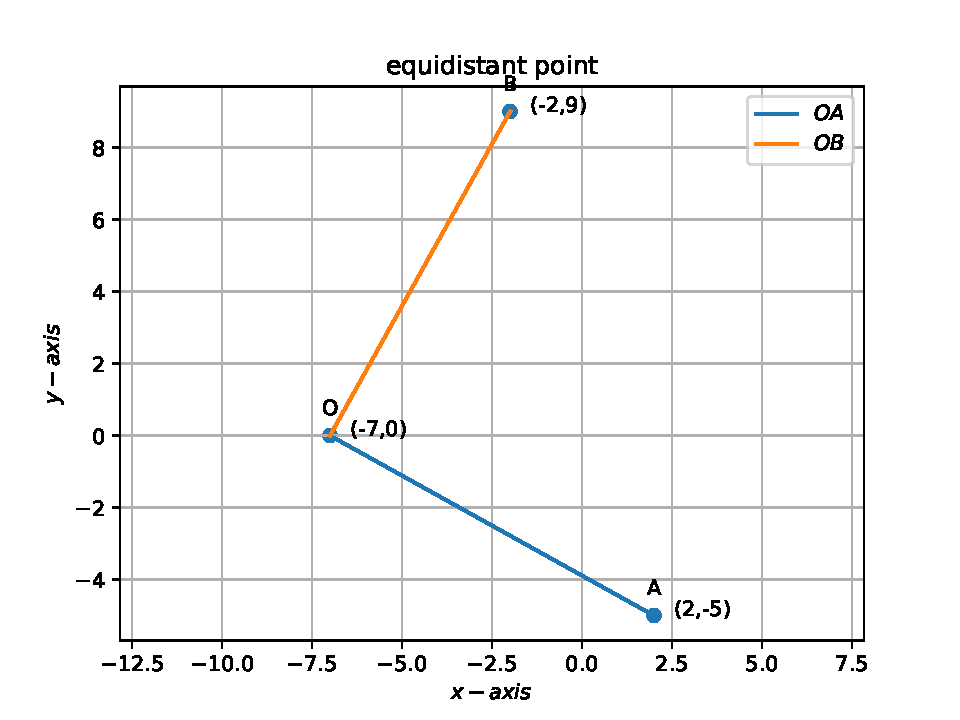
\includegraphics[width=\columnwidth]{chapters/10/7/1/7/figs/fig.pdf}
 \end{center}
\caption{}
\label{fig:10/7/1/7Fig1}
\end{figure}


\item Find the values of $y$ for which the distance between the points                  $\vec{P}(2,-3)$ and $\vec{Q}(10,y)$ is 10 units.
\item  If $\vec{Q}(0, 1)$ is equidistant from $\vec{P}(5, -3)$ and $\vec{R}(x, 6)$, find the values of $x$. Also find the
distances $QR$ and $PR$.
\item  Find a relation between $x$ and $y$ such that the point $(x,y)$ is equidistant from the point
$(3, 6)$ and $(– 3, 4)$.
	\\
\solution
		\iffalse
\documentclass[12pt]{article}
\usepackage{graphicx}
%\documentclass[journal,12pt,twocolumn]{IEEEtran}
\usepackage[none]{hyphenat}
\usepackage{graphicx}
\usepackage{listings}
\usepackage[english]{babel}
\usepackage{graphicx}
\usepackage{caption} 
\usepackage{hyperref}
\usepackage{booktabs}
\def\inputGnumericTable{}
\usepackage{color}                                            %%
    \usepackage{array}                                            %%
    \usepackage{longtable}                                        %%
    \usepackage{calc}                                             %%
    \usepackage{multirow}                                         %%
    \usepackage{hhline}                                           %%
    \usepackage{ifthen}
\usepackage{array}
\usepackage{amsmath}   % for having text in math mode
\usepackage{listings}
\lstset{
language=tex,
frame=single, 
breaklines=true
}
  
%Following 2 lines were added to remove the blank page at the beginning
\usepackage{atbegshi}% http://ctan.org/pkg/atbegshi
\AtBeginDocument{\AtBeginShipoutNext{\AtBeginShipoutDiscard}}
%


%New macro definitions
\newcommand{\mydet}[1]{\ensuremath{\begin{vmatrix}#1\end{vmatrix}}}
\providecommand{\brak}[1]{\ensuremath{\left(#1\right)}}
\providecommand{\norm}[1]{\left\lVert#1\right\rVert}
\newcommand{\solution}{\noindent \textbf{Solution: }}
\newcommand{\myvec}[1]{\ensuremath{\begin{pmatrix}#1\end{pmatrix}}}
\let\vec\mathbf

\begin{document}

\begin{center}
\title{\textbf{Coordinate Geometry}}
\date{\vspace{-5ex}} %Not to print date automatically
\maketitle
\end{center}

\setcounter{page}{1}



\begin{enumerate}

\item\textbf{Problem statement :} Find a relation between x and y such that the point $\myvec{x ,y}$ is equidistant from the point $\myvec{3 ,6}$ and $\myvec{-3 ,4}$

\solution \\
\textbf{\centering{Method I}}
\fi
The input parameters for this problem are given as
	\begin{align}
	\vec{P} = \myvec{
		x\\
		y\\
		},
	\vec{A} = \myvec{
		3\\
		6\\
		},
        \vec{B} = \myvec{
		3\\
		-4\\
		}
	\end{align}
\iffalse

  If $\vec{P}$ equidistant from the points $\vec{A}$ and $\vec{B}$, 
\begin{align}
 \norm{\vec{P}-\vec{A}} &=
\norm{\vec{P}-\vec{B}} 
\\
 \implies \norm{\vec{P}-\vec{A}}^2 &=
\norm{\vec{P}-\vec{B}}^2 
\end{align}
which can be expressed as 
\begin{align}
%  \label{eq:chapters/10/7/1/10/norm2d_dist}
 \brak{\vec{P}-\vec{A}}^{\top} \brak{\vec{P}-\vec{A}}=
 \brak{\vec{P}-\vec{B}}^{\top} 
\brak{\vec{P}-\vec{B}}
\\
 \implies \norm{\vec{P}}^2-2{\vec{P}}^{\top}\vec{A} + \norm{\vec{A}}^2
 \\= \norm{\vec{P}}^2-2{\vec{P}}^{\top}\vec{B} + \norm{\vec{B}}^2
\end{align}
which can be simplified to obtain
%  \eqref{eq:chapters/10/7/1/10/norm2d_equidist}.
  \fi
  \begin{align}
   \vec{P} =
    y\vec{e}_1
  \end{align}
  where 
  \begin{align}
   y &=\frac{\norm{\vec{A}}^2 -\norm{\vec{B}}^2 }{2\brak{\vec{A}-\vec{B}}^{\top }\vec{e}_1
}\label{eq:chapters/10/7/1/10/5}  
  \end{align}
  Substituting the $\vec{A}, \vec{B}$ values in \eqref{eq:chapters/10/7/1/10/5},
\begin{align}
 \brak{\vec{A}-\vec{B}}=
 \myvec{6 \\ 2},
   \norm{\vec{A}}^2 = 45,
   \norm{\vec{B}}^2 = 25
    \end{align}
    yielding
$y =  5$.
Hence, 
\begin{align}
\vec{P} = \myvec{ 0 \\ 5}
\end{align}
%
See Fig. 
\ref{fig:chapters/10/7/1/10/Fig1}.
\begin{figure}[!h]
 \begin{center}
  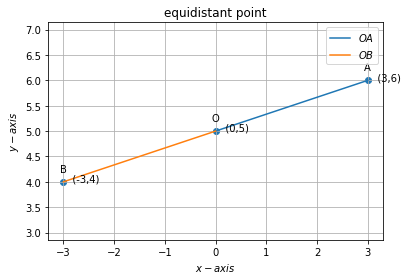
\includegraphics[width=\columnwidth]{./chapters/10/7/1/10/figs/fig.png}
 \end{center}
\caption{}
\label{fig:chapters/10/7/1/10/Fig1}
\end{figure}



\end{enumerate}

